\documentclass[12pt,letterpaper, onecolumn]{exam}
\usepackage{amsmath}
\usepackage{amssymb}
\usepackage[lmargin=71pt, tmargin=1.2in]{geometry}  %For centering solution box
\usepackage{graphicx}
\lhead{Term Paper\\}
\rhead{Image Recognition\\}
% \chead{\hline} % Un-comment to draw line below header
\thispagestyle{empty}   %For removing header/footer from page 1
\begin{document}

\begingroup  
    \centering
    \LARGE TERM PAPER\\
    \LARGE ARTIFICIAL INTELLIGENCE\\[0.5em]
    \large \today\\[0.5em]
    \large Image Recognition and Monitoring using python\par
    \large Roll Number - 19111026\par
    \large BME/ 5th sem / B.Tech\par
\endgroup
\rule{\textwidth}{0.4pt}
\pointsdroppedatright   %Self-explanatory
\printanswers
\renewcommand{\solutiontitle}{\noindent\textbf{Ans:}\enspace}   %Replace "Ans:" with starting keyword in solution box


    \section{Introduction}
    Image recognition in python gives an input image to a Neural network (the most popular neural network used for image recognition is Convolution Neural Network). \\\\
  This is the main focus of our article that will be discussed in detail shortly.\\
  The task is split mainly into two categories:
\\\\
  1. Classification of the image to a single category /multiple categories.
\\\\
  2. Identification of certain objects in an Image ( This can be done only for the purpose of detection, segmentation, object tracking in videos, etc..)
  \\\\
  Though final Tasks are different but the algorithm used in the neural network is the same.
  \\\\\\

    \section{Layers in recognition}
    The Input image consists of pixels. If it is a grayscale Image (B/W Image), it is displayed as a 2D array, and each pixel takes a range of values from 0 to 255. If it is RGB       Image (coloured Image), it is transformed into a 3D array where each layer represents a colour.\\\\\\
    
    \subsection{Convolutional layer:}
    Purpose: Detect certain features in the image.\\\\\\

  Operation: The convolution of Input Image and feature detector (or filter) is used to detect certain features in the image. Convolution occurs in the same manner as digital      signal processing. Convolution occurs in the same manner as digital signal processing. Feature detector values can be predetermined if you know what features to extract from   the image, or values can be initialized randomly, and the network training process determines the best filter values that fit our model.
\\\\
  Output: The output of this layer is called a feature map. The size of the feature map is less than the size of the image. This has the advantage of making the computation        process easier. A point to elaborate is that part of image information is lost due to decreased output size. However, this doesn’t cause a problem because the feature map’s      values are different from the original image as they represent the locations where the highest detection of the filter is performed.\\\\\\
    
    \subsection{Relu rectifier:}
    Purpose: increase non-linearity of images so they can be easily separable. Normally, images are highly non-linear because there are many details related to intensity, borders,   etc. The convolutional layer can result in linear feature maps, so this step is highly crucial.\\\\

  Operation: A relu rectifier is applied to the feature map
\\\\
  Output: The output of this layer is a feature map with higher non-linearity.\\\\\\
  \subsection{ Maximum Pooling layer:}
    Purpose: Distinguish features if they are distorted. The main purpose is to detect features even if there is a slight difference in the feature itself.\\\\

  Operation: Maximum pooling finds the maximum value of a certain window. The maximum pooling Layer shifts to the left by a certain number of steps called strides.\\\\

  Output: Output of this layer is pooled feature map. Pooled feature map has multiple advantages. The output size is always smaller. Maximum values are still present, and these    are the locations of highest similarity with the featured filter. In addition, more than 75\% of image information that isn’t related to features or is useless are removed. In    addition, the Feature map becomes prominent to distortion if the feature value is shifted from its location.
 \\\\
  Convolutional and MaxPool layers can be repeated more than once according to our machine learning problem. Then, We add MLP to the existing CNN. The main purpose of this step    is to increase the number of feature attributes to make better class predictions.\\\\\\
  
  \subsection{Flattening}
  Numbers are taken row by row, column by column and put in a single column. The main purpose of this step is to convert matrix output from the previous layer to a format that     can be accepted by ANN.\\\\\\
  \subsection{Fully Connected Layer}
  This is an artificial neural network where input is the flattened layer, followed by a group of fully connected layers—finally, the output layer according to categories that     we have or objects that need to be detected.
  
  \section{PROGRAMMING LANGUAGES AND LIBRARIES MAINLY USED IN IMAGE RECOGNITION}
  There are many programming languages that are used in today's world for image recognition and monitoring systems. According to ranking they are:\\
  1)Python - highly used for its fast performance and immense amount of libraries\\
  2)C/C++ - second most used language for image recognition due its speed.\\
  3)Java \\
  4)Matlab - mainly used in monitoring systems\\
  \\\\
  libraries mainly used for the process are:\\
  1)Open-CV\\
  2)Sci-kit image\\
  3)Sci-py\\
  4)Pillow/Pil\\
  5)Numpy\\
  6)Mahotas\\
  7)SimpleITK\\
  8)Pgmagick\\
  \\
  Other Libraries used in the process are:
  1)pandas\\
  2)Matplotlib\\
  3)Seaborn\\
  4)os
  
  \section{How does image recognition work?}
    The following steps are done in the process of image recognition
    \subsection{Step 1}
        First, a great number of characteristics, called features are extracted from the image. An image is actually made of “pixels”.
        Each pixel is represented by a number or a set of numbers — and the range of these numbers is called the color depth (or bit depth). In other words, the color depth indicates the maximum number of potential colors that can be used in an image. In an (8-bit) greyscale image (black and white) each pixel has one value that ranges from 0 to 255. Most images today use 24-bit color or higher. An RGB color image means the color in a pixel is the combination of red, green and blue. Each of the colors ranges from 0 to 255.So a pixel contains a set of three values RGB(102, 255, 102) refers to color \#66ff66. An image 800 pixel wide, 600 pixels high has 800 x 600 = 480,000 pixels = 0.48 megapixels (“megapixel” is 1 million pixels). An image with a resolution of 1024×768 is a grid with 1,024 columns and 768 rows, which therefore contains 1,024 × 768 = 0.78 megapixels.
        
        \begin{figure}[htp]
            \centering
            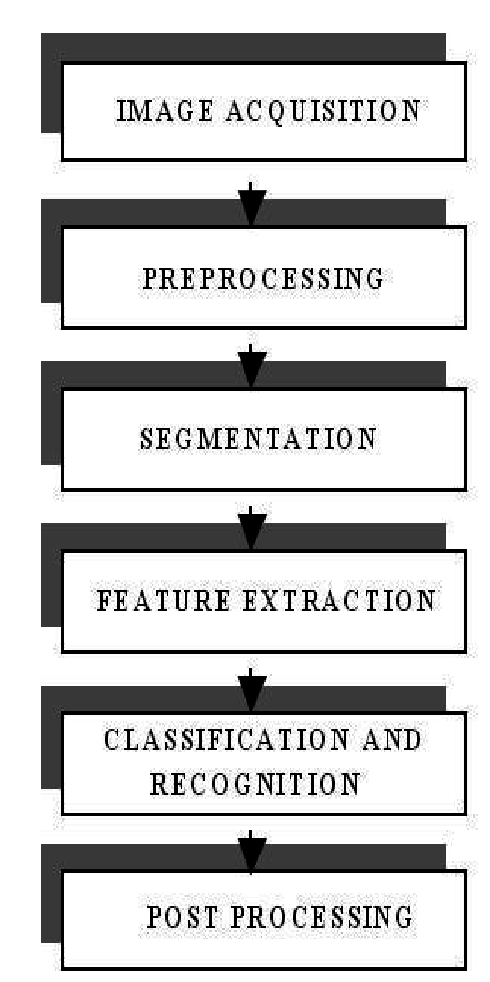
\includegraphics[width=4cm]{image_1}
            \label{fig:steps}
        \end{figure}

    \subsection{Step 2}
        Once each image is converted to thousands of features, with the known labels of the images we can use them to train a model. Figure (B) shows many labeled images that belong to different categories such as “dog” or “fish”. The more images we can use for each category, the better a model can be trained to tell an image whether is a dog or a fish image. Here we already know the category that an image belongs to and we use them to train the model. This is called supervised machine learning.
    \subsection{Step 3}
        Training the data requires labelled data which is then convreted into pixels and the fed into deep neural networks for processing.The huge networks in the middle can be considered as a giant filter. The images in their extracted forms enter the input side and the labels are in the output side. The purpose here is to train the networks such that an image with its features coming from the input will match the label in the right.
    
    \subsection{Step 4}
    Once a model is trained, it can be used to recognize (or predict) an unknown image.
    The new image will also go through feature extraction process.
    
    \begin{figure}[htp]
            \centering
            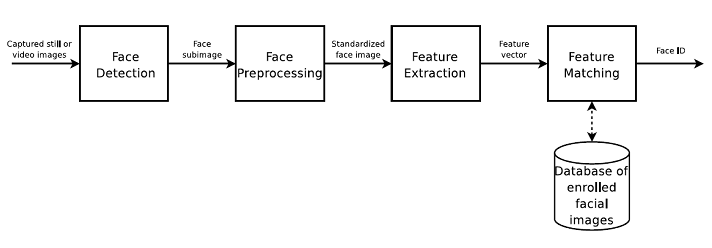
\includegraphics[width=15cm]{image_2}
            \label{fig:steps}
        \end{figure}
    
\section{DEEP IMAGE SCALING UP IMAGE RECOGNITION }
    Deep Image, developed using end-to-end deep learning. The key components are a custom-built supercomputer dedicated to deep learning, a highly optimized parallel algorithm using new strategies for data partitioning and communication, larger deep neural network models, novel data augmentation approaches, and usage of multi-scale high-resolution images.
    
    \subsection{Hardware/Software Co-design }
    It is clear that different classes of algorithms would perform differently on different computing architectures. Graphic processors, or GPUs, often perform extremely well for compute-intensive algorithms. Early work shows that for clustering algorithms, a single GPU offers 10x more performance than top-of-the-line 8 cores workstations, even on very large datasets with more than a billion data points. 
    
    \subsection{Optimization }
    The previous work mainly focuses on a single server with multiple GPUs or small GPU clusters, so it's hard to extend directly to a large GPU cluster because of the communication bottlenecks. In our work, we focus on optimizing parallel strategies, minimizing data transfers and overlapping the computation and communications. This is needed for approaching the peak performance for the large supercomputers like Minwa. 
    
    \subsection{Data Parallelism}
    In one forward-backward pass, the parameters and gradients of all layers are copied on every GPU. All GPUs compute gradients based on local training data and a local copy of weights. They then exchange gradients and update the local copy of weights.\\
    \\
    Two strategies have helped us to achieve better parallelism. The first one is the ‘butterfly synchronization’ strategy, in which all gradients are partitioned into K parts and each GPU is responsible for its own part.\\\\
    Another is the ‘lazy update’ strategy. Once the gradients are generated in the backward pass, each GPU sends its generated gradient to the corresponding GPUs in an asynchronous way. 
    
    \subsection{Model-Data Parallelism}
    While data parallelism works well for the smaller models. It does not work if the model size cannot be fit into the memory of a single GPU. Model-data parallelism is used to address this problem. Here, data parallelism is still used at convolutional layers but fully-connected layers are instead partitioned and distributed to multiple GPUs. This works  because convolutional layers have fewer parameters but more computation. 
    
    \subsection{Scaling Efficiency}
    Testing the scaling efficiency by training a model for an image classification task. The network has 8 convolutional layers and 3 fully-connected layers followed by a 1000- way softmax. Measured by the epoch time, the scalability efficiency and the speedup of going through images are shown in Figure 2. For the convenience of observing the scalability of different parallel strategies, we fixed the number of images processed by each GPU to 64 (slices = 64). The time taken for hybrid parallelism and data parallelism with different numbers of GPUs is shown in Figure 2(a). The data parallelism performs better when the involved GPU number is larger than 16. This is because communication overhead of the data parallel strategy is constant when the size of model is fixed. The speedup is larger with larger batch size . Compared with a single GPU, a 47x speedup of going through images is achieved by using 64 GPUs with a minibatch size of 1024. As the number of GPUs increases, the total device memory is also increasing, and more data can be cached on the device memory. This is helpful for improving parallel efficiency.
    
    \section{Advantages and disadvantages}
    \subsection{Compared to other biometric systems}
    One key advantage of a facial recognition system that it is able to perform mass identification as it does not require the cooperation of the test subject to work. Properly designed systems installed in airports, multiplexes, and other public places can identify individuals among the crowd, without passers-by even being aware of the system. However, as compared to other biometric techniques, face recognition may not be most reliable and efficient. Quality measures are very important in facial recognition systems as large degrees of variations are possible in face images. Factors such as illumination, expression, pose and noise during face capture can affect the performance of facial recognition systems. Among all biometric systems, facial recognition has the highest false acceptance and rejection rates,thus questions have been raised on the effectiveness of face recognition software in cases of railway and airport security
    
    \subsection{Weaknesses}
    Face recognition is less effective if facial expressions vary. A big smile can render the system less effective. For instance: Canada, in 2009, allowed only neutral facial expressions in passport photos.\\
    There is also inconstancy in the datasets used by researchers. Researchers may use anywhere from several subjects to scores of subjects and a few hundred images to thousands of images. It is important for researchers to make available the datasets they used to each other, or have at least a standard dataset.\\
    Facial recognition systems have been criticized for upholding and judging based on a binary gender assumption.When classifying the faces of cisgender individuals into male or female, these systems are often very accurate, however were typically confused or unable to determine the gender identity of transgender and non-binary people. Gender norms are being upheld by these systems, so much so that even when shown a photo of a cisgender male with long hair, algorithms was split between following the gender norm of males having short hair, and the masculine facial features and became confused.
    
    \subsection{Ineffectiveness}
    Systems are often advertised as having accuracy near 100\%; this is misleading as the studies often use much smaller sample sizes than would be necessary for large scale applications. Because facial recognition is not completely accurate, it creates a list of potential matches. A human operator must then look through these potential matches and studies show the operators pick the correct match out of the list only about half the time. This causes the issue of targeting the wrong suspect.
\section{Emotion recognition}
In the 18th and 19th century the belief that facial expressions revealed the moral worth or true inner state of a human was widespread and physiognomy was a respected science in the Western world. From the early 19th century onwards photography was used in the physiognomic analysis of facial features and facial expression to detect insanity and dementia. In the 1960s and 1970s the study of human emotions and its expressions was reinvented by psychologists, who tried to define a normal range of emotional responses to events. The research on automated emotion recognition has since the 1970s focused on facial expressions and speech, which are regarded as the two most important ways in which humans communicate emotions to other humans. In the 1970s the Facial Action Coding System (FACS) categorization for the physical expression of emotions was established. Its developer Paul Ekman maintains that there are six emotions that are universal to all human beings and that these can be coded in facial expressions. Research into automatic emotion specific expression recognition has in the past decades focused on frontal view images of human faces.

\section{Anti-facial recognition systems}
In January 2013 Japanese researchers from the National Institute of Informatics created 'privacy visor' glasses that use nearly infrared light to make the face underneath it unrecognizable to face recognition software. The latest version uses a titanium frame, light-reflective material and a mask which uses angles and patterns to disrupt facial recognition technology through both absorbing and bouncing back light sources.Some projects use adversarial machine learning to come up with new printed patterns that confuse existing face recognition software.\\
Another method to protect from facial recognition systems are specific haircuts and make-up patterns that prevent the used algorithms to detect a face, known as computer vision dazzle. Incidentally, the makeup styles popular with Juggalos can also protect against facial recognition.
\\
Facial masks that are worn to protect from contagious viruses can reduce the accuracy of facial recognition systems. A 2020 NIST study tested popular one-to-one matching systems and found a failure rate between five and fifty percent on masked individuals. The Verge speculated that the accuracy rate of mass surveillance systems, which were not included in the study, would be even less accurate than the accuracy of one-to-one matching systems. The facial recognition of Apple Pay can work through many barriers, including heavy makeup, thick beards and even sunglasses, but fails with masks.
    
\section{Refrences}
www.wikipedia.org
www.scholar.google.com
www.sciencedirect.com
ieeexplore.ieee.org

\end{document}
